%================================================================%
%=============  Modelo de Trabalho de Conclusão de curso ========%
%========================  IFMG =================================% 
% AUTORES:
% prof. Elias J R Freitas =======================================%
% ej-ensino.com.br
%
% baseado no modelo DEPRO-UFOP 
% estrutura elaborada inicialmente por
% Marcelus Xavier Oliveira  e Dayanne Gouveia Coelho ===============%

%================================================================%
% Proposta de texto em conformidade com normas da ABNT ----------%
% Modelo em conformidade com 
% Manual de Normalização de Trabalhos Acadêmicos 21/02/2020
% https://www.ifmg.edu.br/portal/ensino/bibliotecas/
% arquivos-bibliotecas/copy_of_ManualdeNormalizaoIFMG2020.pdf
% implementadas pelo projeto abntex2, que pode ser acessado pela %
% página  http://abntex2.googlecode.com/  -----------------------%
%================================================================%

%================================================================%
% Versao abntex2
%======================== Versão 2022/02 ========================%
%================================================================%


\documentclass[12pt, % tamanho da fonte
	%openright,	% capítulos começam em pág ímpar
	oneside, %para impressão apenas em um lado (formato digital).  		  
	% twoside, %para impressão em frente e verso.  
	a4paper,			% tamanho do papel. 
	english,			% Idioma adicional para hifenização
	brazilian			% Idioma principal 
	]{packages/abntex2-ifmg}
	
%------------------------------------------------------------
%------------    Estrutura do texto   -----------------------         

% Pacotes Básicos:
%\usepackage{lmodern}			    % Usa a fonte Latin Modern			
\usepackage{pslatex}                % Usa a fonte Times New Roman
\usepackage[T1]{fontenc}		  % Selecao de codigos de fonte.
\usepackage[utf8]{inputenc}		% Codificacao do documento (conversão automática dos acentos)
\usepackage{lastpage}			    % Usado pela Ficha catalográfica
\usepackage{indentfirst}		  % Indenta o primeiro parágrafo de cada seção.
\usepackage[table]{xcolor}
\usepackage{color}				    % Controle das cores
\usepackage{graphicx}			    % Inclusão de gráficos
\usepackage{microtype} 		  	% para melhorias de justificação

\usepackage{tablefootnote} % para colocar footnotes em tabelas e figuras

% Pacotes Extras:
\usepackage[final]{pdfpages}
\usepackage{amsmath,amsthm}   %Símbolos Matemáticos
\usepackage{indentfirst} % Indenta primeiro parágrafo 
\usepackage[portuguese, ruled, linesnumbered,commentsnumbered, algo2e, vlined, lined, boxed, algochapter]{algorithm2e} % Algoritmos 
\usepackage{hyperref}
\usepackage[brazilian,hyperpageref]{backref}	 % Paginas com as citações na bibliograficas
\usepackage{tabularx}
\usepackage{array}


%\usepackage[num]{abntex2cite}	% Citações padrão ABNT númerico
\usepackage[alf,abnt-emphasize=bf,abnt-full-initials=no,abnt-etal-list=5,abnt-etal-text=emph,abnt-repeated-author-omit=yes]{abntex2cite}
%\usepackage[alf,abnt-emphasize=bf,abnt-etal-list=0,abnt-etal-text=emph]{abntex2cite}

% se desejar justificar as referências (pela abnt é alinhado a esquerda)
% \usepackage[alf,abnt-emphasize=bf,bibjustif]{abntex2cite}

\usepackage{float} % para ajustar a posição das imagens

\usepackage{tikzsymbols} %para caracteres emoji
\usepackage{stackengine}
\usepackage{scalerel}

\newcommand\dangersign[1][2ex]{%
  \renewcommand\stacktype{L}%
  \scaleto{\stackon[1.3pt]{\color{red}$\triangle$}{\tiny\bfseries !}}{#1}%
}

\usepackage{etoolbox}
%\usepackage[num]{abntex2cite}  % Citações numéricas

\usepackage{lipsum}

%para usar os algoritmos e matematica
\newcommand{\var}{\texttt}

\usepackage{amssymb}
\usepackage{amsmath}



% Defininfo Cores:
\definecolor{blue}{RGB}{25,25,112}
\definecolor{midgray}{gray}{.7}

\makeatletter % informações do PDF
\hypersetup{ % pagebackref=true,
	pdftitle={\@title}, 
	pdfauthor={\@author},
    pdfsubject={\imprimirpreambulo},
	pdfcreator={LaTeX with abnTeX2},
	pdfkeywords={abnt}{latex}{abntex}{abntex2}{trabalho acadêmico}, 
	colorlinks=true,     % false: boxed links; true: colored links
    linkcolor=black,          	% color of internal links
    citecolor=black,        		% color of links to bibliography
    filecolor=magenta,      	% color of file links
    urlcolor=black,
	bookmarksdepth=4 }
\makeatother
 

% -------------------------------------------- 
% Espaçamentos entre linhas e parágrafos 
\setlength{\parindent}{1.3cm} % O tamanho do parágrafo

% Controle do espaçamento entre um parágrafo e outro:
\setlength{\parskip}{0.2cm}  % tente também \onelineskip

% Definição de ambientes matemáticos em português 
\newtheorem{teorema}{Teorema}[chapter]
\newtheorem{axioma}{Axioma}[chapter]
\newtheorem{corolario}{Corolário}[chapter]
\newtheorem{lema}{Lema}[chapter]
\newtheorem{proposicao}{Proposição}[chapter]
\newtheorem{definicao}{Definição}[chapter]
\newtheorem{exemplo}{Exemplo}[chapter]
\newtheorem{observacao}{Observação}[chapter]

% Novos Comandos
\usepackage{tgtermes}
\renewcommand{\ABNTEXchapterfont}{\rmfamily\bfseries}

% Variáveis adicionais
\providecommand{\imprimirautorcite}{}
\newcommand{\autorcite}[1]{\renewcommand{\imprimirautorcite}{#1}} 
\providecommand{\imprimirsigla}{}
\newcommand{\sigla}[1]{\renewcommand{\imprimirsigla}{#1}}
\providecommand{\imprimiruf}{}
\newcommand{\uf}[1]{\renewcommand{\imprimiruf}{#1}}
\providecommand{\imprimircurso}{}
\newcommand{\curso}[1]{\renewcommand{\imprimircurso}{#1}}
\providecommand{\imprimirinstituto}{}
\newcommand{\instituto}[1]{\renewcommand{\imprimirinstituto}{#1}}
\providecommand{\imprimirdepartamento}{}
\newcommand{\departamento}[1]{\renewcommand{\imprimirdepartamento}{#1}}
\providecommand{\imprimirano}{}
\newcommand{\ano}[1]{\renewcommand{\imprimirano}{#1}}
\providecommand{\imprimirdia}{}
\newcommand{\dia}[1]{\renewcommand{\imprimirdia}{#1}}
\providecommand{\imprimirmes}{}
\newcommand{\mes}[1]{\renewcommand{\imprimirmes}{#1}}
\providecommand{\imprimirgrau}{}
\newcommand{\grau}[1]{\renewcommand{\imprimirgrau}{#1}}
\providecommand{\imprimirexaminadorum}{}
\newcommand{\examinadorum}[1]{
    \renewcommand{\imprimirexaminadorum}{#1}}
\providecommand{\imprimirexaminadordois}{}
\newcommand{\examinadordois}[1]{
    \renewcommand{\imprimirexaminadordois}{#1}}
\providecommand{\imprimirexaminadortres}{}
\newcommand{\examinadortres}[1]{
    \renewcommand{\imprimirexaminadortres}{#1}}
\providecommand{\imprimirexaminadorquatro}{}
\newcommand{\examinadorquatro}[1]{
    \renewcommand{\imprimirexaminadorquatro}{#1}}
\providecommand{\imprimirttorientador}{}
\newcommand{\ttorientador}[1]{
    \renewcommand{\imprimirttorientador}{#1}} 
\providecommand{\imprimirttcoorientador}{}
\newcommand{\ttcoorientador}[1]{
    \renewcommand{\imprimirttcoorientador}{#1}}
\providecommand{\imprimirttexaminadorum}{}
\newcommand{\ttexaminadorum}[1]{
    \renewcommand{\imprimirttexaminadorum}{#1}}
\providecommand{\imprimirttexaminadordois}{}
\newcommand{\ttexaminadordois}[1]{\renewcommand{
        \imprimirttexaminadordois}{#1}}
\providecommand{\imprimirttexaminadortres}{}
\newcommand{\ttexaminadortres}[1]{
    \renewcommand{\imprimirttexaminadortres}{#1}}
\providecommand{\imprimirttexaminadorquatro}{}
\newcommand{\ttexaminadorquatro}[1]{
    \renewcommand{\imprimirttexaminadorquatro}{#1}}

% Cria o comando \subtitulo. A norma define que o TITULO deve ser em caixa alta
% negrito, mas o subtitulo deve ser em caixa baixa.
\providecommand{\imprimirsubtitulo}{}
\newcommand{\subtitulo}[1]{\renewcommand{\imprimirsubtitulo}{#1}}

%----------------------------------------------------
\renewcommand{\imprimircapa}{  % Capa 
\begin{capa}
%\begin{center}
\includegraphics[scale=1]{Figuras/ifmg.png}\end{center}
\begin{center}{
             \large \MakeTextUppercase{\imprimirinstituicao} - \MakeTextUppercase{\imprimirinstituto} \\
              %\imprimirdepartamento \\
              \MakeTextUppercase{Bacharelado em \imprimircurso} \\
              \vspace{2cm}
			  \large {\imprimirautor} 
			  }\end{center}
\vfill
        \begin{center}
        \MakeTextUppercase{\large \textbf{\imprimirtitulo}}
        \MakeTextLowercase{\textbf{\imprimirsubtitulo}}
				\vspace{2cm}
				%{\large \imprimirautor} 	
				\vfill
        {\large{\imprimirlocal \\ \imprimirano }}
        \end{center}
\end{capa}   } % Capa

%----------------------------------------------------
\renewcommand{\imprimirfolhaderosto}{% folha de rosto
    \begin{center}
    {{\MakeTextUppercase \imprimirautor}}  \\
		\vfill
		\large {\textbf{\MakeTextUppercase{\imprimirtitulo}}
        \MakeTextLowercase{\textbf{\imprimirsubtitulo}}}
    \end{center}
    \vfill 
    \begin{flushright} 
    \parbox{0.6\linewidth}{
		\imprimirtipotrabalho~ apresentado à banca examinadora do curso de \imprimircurso~ do \imprimirinstituicao~\imprimirinstituto, como parte dos requisitos para obtenção do título de \imprimirgrau. \\
		\vfill
		\textbf{\imprimirorientadorRotulo}~\imprimirorientador \\
		\vfill 
		\textbf{\imprimircoorientadorRotulo}~\imprimircoorientador}
   \end{flushright} 
   
	 \vfill
   \begin{center}
   {\large{\imprimirlocal \\ \imprimirano}}
   \end{center} }  % folha de rosto

%----------------------------------------------------


%================================================================================
% Pacotes de citações
%================================================================================

% Configurações do pacote backref
% Texto padrão antes do número das páginas
\renewcommand{\backref}{}
% Define os textos da citação
\addto\captionsbrazil{% portugues-brasil
    % Usado sem a opção hyperpageref de backref
    \renewcommand{\backrefpagesname}{Citado na(s) p{\'a}gina(s):~}
    \renewcommand*{\backrefalt}[4]{
    	\ifcase #1 %
    		Nenhuma cita{\c c}{\~a}o no texto.%
    	\or
    		Citado na p{\'a}gina #2.%
    	\else
    		Citado #1 vezes nas p{\'a}ginas #2.%
    	\fi}%
}
\addto\captionsenglish{% ingles
    % Usado sem a opção hyperpageref de backref
    \renewcommand{\backrefpagesname}{Cited on page(s):~}
    \renewcommand*{\backrefalt}[4]{
    	\ifcase #1 %
    		No citation.%
    	\or
    		Cited on page #2.%
    	\else
    		Cited #1 times on pages #2.%
    	\fi}%
}
% ---
\makeatletter
\newcommand\thefontsize{Fonte tamanho: \f@size pt}
\makeatother



% para não deixar uma figura sozinha no centro de uma página,
% mas no topo da página.tabularx
\makeatletter
\setlength{\@fptop}{0pt}
\makeatother




%--  % Estrutura do texto e pacotes principais

% -- Informações para Capa e Folha de Rosto a serem editadas

\titulo{Aplicação Low-Code em Mendix para o Registro e o Acompanhamento do QRQC:}
\subtitulo{um estudo de caso em ambiente industrial}

\autor{Brunny Augusto Gumieri Silva} \autorcite{SILVA, Brunny Augusto Gumieri}
\local{Betim}
\data{\rule{1cm}{0.15mm} de \rule{1cm}{0.15mm} de \rule{1cm}{0.15mm}} 
\dia{\rule{1cm}{0.15mm}} \mes{\rule{1cm}{0.15mm}} 
\ano{2026}
\orientador{Prof. Me. Virgil Del Duca Almeida}  % Nome do orientador 
\ttorientador{IFMG} % Instituição do orientador
% \coorientador{Prof. Me. XXXXXXXXX}   % Nome do coorientador
% \ttcoorientador{IFMG} % Instituição do Coorientador
\instituicao{Instituto Federal de Educação, Ciência e Tecnologia de Minas Gerais} \sigla{IFMG}
\instituto{\textit{Campus} Betim}
%\departamento{Departamento de Engenharia de Controle e Automação e Técnicas Fundamentais}
\curso{Engenharia de Controle e Automação}	
\tipotrabalho{Trabalho de Conclusão de Curso}
\grau{Bacharel em Engenharia de Controle e Automação}

%------Nomes dos examinadores.  
% Preencher os examinadores quando a banca for definida.
% \examinadorum{Prof. Dr. Nome do examinador} \ttexaminadorum{Instituição}
% \examinadordois{Prof. Dr. Nome do examinador} \ttexaminadordois{Instituição}
%\examinadortres{Prof. Dr. Membro da Banca  3} \ttexaminadortres{Universidade Federal de ... - UFXX}
%\examinadorquatro{Prof. Dr. Membro da Banca  4} \ttexaminadorquatro{Universidade Federal de ... - UFXX}

% ------------------------------------------------------
% Índice remissivo não utilizado.   

\begin{document} % Início do documento

\hypersetup{hidelinks} % remove molduras coloridas dos hiperlinks no PDF

\frenchspacing  % Retira espaço obsoleto entre as frases.

% ----------------------------------------------------------
% -- Elementos Pré-Textuais: -------------------------------
\hypersetup{pageanchor=false}
\imprimircapa  % Capa
\hypersetup{pageanchor=true}
\pagenumbering{arabic}
\setcounter{page}{1} % A contagem começa na folha de rosto
\imprimirfolhaderosto % Folha de rosto

% Inserir a ficha catalográfica e a folha de aprovação oficiais na versão final.
% % ---------------------------------------------------------------
% ----------------  Ficha Catalográfica  -------------------------
% ---------------------------------------------------------------
% Modelo de ficha catalográfica. Você deverá substituir esta
% folha na versão final da monografia por um pdf fornecido pela 
% biblioteca. Salve o modelo oficial como ficha_catalografica.pdf
% e use o comando abaixo para inseri-lo na versão final do texto.

%\begin{fichacatalografica}
%    \includepdf{ficha_catalografica.pdf}
%\end{fichacatalografica}



%% Modelo de Como fazer a Ficha Catalográfica:

\begin{fichacatalografica}
	\begin{center}					% Minipage Centralizado
	 \large {(Página onde será inserida a ficha catalográfica- Solicitar junto à biblioteca)}
% 	\small
% 	\imprimirautorcite.
% 	%Sobrenome, Nome do autor
	
% 	\hspace{0.5cm}  \\
% 	\imprimirtitulo  / \imprimirautor. --, \imprimirano-
	
% 	\hspace{0.5cm} \pageref{LastPage} p. 1 :il. (colors; grafs; tabs).\\
	
% 	\hspace{0.5cm} \imprimirorientadorRotulo~\imprimirorientador\\
	
% 	\hspace{0.5cm}
% 	\parbox[t]{\textwidth}{\imprimirtipotrabalho~--\\ \imprimirinstituicao. \\
% 	\imprimirinstituto. \\ ~\imprimirdepartamento.}\\
	
% 	\hspace{0.5cm}
% 		1. Palavra-chave1.
% 		2. Palavra-chave2.
% 		2. Palavra-chave3.
% 		I. \imprimirorientador.
% 		II. \imprimirinstituicao.
% 		III. Título 			
	\end{center}
\end{fichacatalografica}



% % ---------------------------------------------------------------
% ----------------  Folha de aprovação  -------------------------
% ---------------------------------------------------------------
% Modelo de Folha de aprovação. Você deverá substituir esta
% folha na versão final da monografia por um pdf fornecido pelo  
% colegiado do seu curso. Salve o modelo oficial como 
% folhadeaprovacao_final.pdf e use o comando abaixo para
% inseri-lo na versão final do texto.

%\begin{fichacatalografica}
%    \includepdf{folhadeaprovacao_final.pdf}
%\end{fichacatalografica} Esta folha será 


\begin{folhadeaprovacao}

\begin{center}
    \large { \imprimirautor}  \\
		\vspace{3cm} 
		\large {\textbf{\MakeTextUppercase{\imprimirtitulo}}~\MakeTextLowercase{\imprimirsubtitulo}}
    \end{center}
    \vspace{2cm}
    \begin{flushright} 
    \parbox{0.6\linewidth}{
		\imprimirtipotrabalho~ apresentado à banca examinadora do curso de \imprimircurso~ do \imprimirinstituicao~\imprimirinstituto, como parte dos requisitos para obtenção do título de \imprimirgrau. \\
		}
   \end{flushright} 
  % \vspace{2cm}
   \vfill
 
   \begin{center}
   \large{
   Aprovado em:~\imprimirdia~/\ \imprimirmes~/\ \imprimirano~ pela banca examinadora:
    \vspace{2cm}
    \vfill
          \rule{15cm}{.1pt} \\
      {\imprimirorientador}~(Orientador)~-~{\imprimirttorientador} 
      \vfill
			 \ifdefvoid{\imprimircoorientador}{}{
      \rule{15cm}{.1pt} \\
      \imprimircoorientador~(Coorientador)~-~\imprimirttcoorientador}
			 \vfill
      \rule{15cm}{.1pt} \\
      {\imprimirexaminadorum}~-~{\imprimirttexaminadorum} %\\ Examinador
        \vfill
        \ifdefvoid{\imprimirexaminadordois}{}{
        \rule{15cm}{.1pt} \\
        \imprimirexaminadordois~-~\imprimirttexaminadordois %\\ Examinador
        }
				\vfill
        \ifdefvoid{\imprimirexaminadortres}{}{
        \rule{15cm}{.1pt} \\
        \imprimirexaminadortres~-~\imprimirttexaminadortres %\\ Examinador
        }
				\vfill
        \ifdefvoid{\imprimirexaminadorquatro}{}{
        \rule{15cm}{.1pt} \\
        \imprimirexaminadorquatro~-~\imprimirttexaminadorquatro %\\ Examinador
        }
   
   }
   \end{center} 

% \begin{center}
%     {\large \textsc{\imprimirautor}} \\
%   	\vspace{2cm}	
%     {\textsc{\Large \textbf{\imprimirtitulo}}} \\
% 		\vspace{2cm}
% \end{center}		

% \noindent \imprimirtipotrabalho~ defendido e aprovado em \imprimirlocal,~ \imprimirdata~,  pela banca examinadora constituída pelos professores:
% \vspace{2cm}
% \begin{center}

%       \rule{10cm}{.1pt} \\
%       {\imprimirorientador} \\ {\imprimirttorientador} \\
% 			 Orientador 
%       \vfill
% 			 \ifdefvoid{\imprimircoorientador}{}{
%       \rule{10cm}{.1pt} \\
%       \imprimircoorientador \\ \imprimirttcoorientador \\ Coorientador }
% 			 \vfill
%       \rule{10cm}{.1pt} \\
%       {\imprimirexaminadorum} \\ {\imprimirttexaminadorum} \\ Examinador
%         \vfill
%         \ifdefvoid{\imprimirexaminadordois}{}{
%         \rule{10cm}{.1pt} \\
%         \imprimirexaminadordois \\ \imprimirttexaminadordois \\ Examinador}
% 				\vfill
%         \ifdefvoid{\imprimirexaminadortres}{}{
%         \rule{10cm}{.1pt} \\
%         \imprimirexaminadortres \\ \imprimirttexaminadortres \\ Examinador}
% 				\vfill
%         \ifdefvoid{\imprimirexaminadorquatro}{}{
%         \rule{10cm}{.1pt} \\
%         \imprimirexaminadorquatro \\ \imprimirttexaminadorquatro \\ Examinador}
% \end{center}
  
\end{folhadeaprovacao}
% ---

% Elementos opcionais: habilitar somente depois de substituir os textos-modelo.
% \begin{dedicatoria}
   \vspace*{\fill}
   \begin{flushright} 
        \parbox{0.6\linewidth}{
		 {
		Dedicatória (opcional).
		}
		}
   \end{flushright} 
   \vspace{2cm}
	 
\end{dedicatoria}
% \begin{agradecimentos}

Agradecimentos (opcional).

\end{agradecimentos}
% \begin{epigrafe}
    \vspace*{\fill}
	\begin{flushright}
	    \parbox{0.6\linewidth}{
		Epígrafe (opcional).
	}
	\end{flushright}
	\vspace{2cm}
\end{epigrafe}
\begin{resumo}
\end{resumo}

\begin{resumo}[ABSTRACT]
\begin{otherlanguage*}{english}
\end{otherlanguage*}
\end{resumo}


\renewcommand{\listfigurename}{LISTA DE ILUSTRA\c{C}\~{O}ES}
\pdfbookmark[0]{\listfigurename}{lof}
\listoffigures*   % Cria a Lista de Figuras
\cleardoublepage

% inserir lista de quadros
% ---
\pdfbookmark[0]{\listofquadrosname}{loq}
\listofquadros*
\cleardoublepage

\pdfbookmark[0]{\listtablename}{lot}
\listoftables*
\cleardoublepage
% ---

% Habilitar quando houver tabelas no trabalho.
% \pdfbookmark[0]{\listtablename}{lot}
% \listoftables*
% \cleardoublepage

%\renewcommand{\listalgorithmcfname}{Lista de algoritmos}
%\pdfbookmark[0]{\listalgorithmcfname}{lof}
%\listofalgorithmes   % Cria a lista de Tabelas
%\cleardoublepage

% ---------------------------------------------------
% ------ Lista de abreviaturas e siglas -------------
% ---------------------------------------------------
\begin{siglas}
  \item[5W2H] Ferramenta de planejamento baseada nas perguntas \textit{What, Why, Where, When, Who, How} e \textit{How much}
  \item[6M] Categorias de causas do Diagrama de Ishikawa: mão de obra, método, máquina, material, medição e meio ambiente
  \item[IFMG] Instituto Federal de Educação, Ciência e Tecnologia de Minas Gerais
  \item[LGPD] Lei Geral de Proteção de Dados Pessoais
  \item[OBA] Auditoria do produto acabado (\textit{Out-of-Box Audit})
  \item[PFMEA] Análise de modos de falha e efeitos do processo (\textit{Process Failure Mode and Effects Analysis})
  \item[QRQC] Resposta Rápida para o Controle da Qualidade (\textit{Quick Response to Quality Control})
  \item[SQL] Linguagem de consulta estruturada (\textit{Structured Query Language})
  \item[TD] Transformação Digital
\end{siglas}

% Habilitar se o trabalho vier a utilizar símbolos que exijam lista própria.
% % ---------------------------------------------------
% ----------- Lista de símbolos ---------------------
% ---------------------------------------------------

\begin{simbolos}
  \item[$ \Gamma $] Letra grega Gama
  \item[$ \Lambda $] Lambda
  \item[$ \zeta $] Letra grega minúscula zeta
  \item[$ \xi$] Letra grega minúscula qsi
  \item[$ \in $] Pertence
\end{simbolos}


\pdfbookmark[0]{\contentsname}{toc}
\tableofcontents*

\cleardoublepage




% ----------------------------------------------------------
% -- Capítulos do Trabalho: --------------------------------
\textual 

%%%%%%%%%%%% ORDEM DOS ARQUIVOS %%%%%%%%%%%%%%%%%%%

\chapter{Introdução} \label{Introducao}

No cenário atual da manufatura, marcado pela competitividade, pela busca por eficiência operacional e pela necessidade de respostas rápidas às demandas produtivas, a digitalização de processos tornou-se relevante para a gestão industrial. A transformação digital está associada ao crescimento e à sobrevivência das organizações, pois envolve o uso de tecnologias digitais para modificar produtos, processos e aspectos organizacionais, promovendo competitividade e geração de valor \cite[p.~1]{terra2022}. No ambiente industrial, essa transformação contribui para o aumento da produtividade, o aprimoramento do controle da qualidade e a ampliação da flexibilidade operacional \cite[p.~1]{ribeiro2026}.

A partir dessa perspectiva, a digitalização não deve ser compreendida apenas como a substituição de registros físicos por meios digitais, mas como uma forma de reorganizar informações e rotinas para apoiar a gestão e a tomada de decisão. A transformação digital nas organizações provoca mudanças em processos produtivos, estrutura organizacional, modelos de negócio, competências, cultura e liderança, desde que alinhada à estratégia corporativa \cite[p.~57]{murici2022}.

Nesse contexto, as plataformas \textit{low code} apresentam-se como recursos capazes de apoiar iniciativas de digitalização ao facilitar o desenvolvimento rápido de aplicações voltadas às necessidades operacionais da organização. Essas plataformas reduzem a dependência de programação manual tradicional, pois utilizam interfaces visuais e elementos pré-configurados para a criação de aplicações, permitindo maior agilidade, menor complexidade e maior participação dos usuários ligados ao negócio no desenvolvimento de soluções digitais \cite[p.~2]{sanchis2020}.

A relevância dessas plataformas pode ser observada na pesquisa apresentada por \citeonline[p.~3]{sanchis2020}, baseada em um levantamento realizado com mais de 3.300 profissionais de tecnologia da informação em diferentes continentes. Conforme apresentado na Figura~\ref{fig:motivos-low-code}, 66\% dos respondentes indicaram a aceleração da transformação digital e o aumento da capacidade de resposta às demandas do negócio como os principais motivos para o uso de plataformas \textit{low code}. Além disso, 45\% destacaram a redução da dependência de competências técnicas difíceis de contratar.

Esses resultados são relevantes para este estudo porque aproximam o uso de plataformas \textit{low code} das necessidades práticas observadas em ambientes industriais, nos quais a agilidade no desenvolvimento de soluções, a redução de registros manuais e a maior disponibilidade de informações podem contribuir para a melhoria da gestão operacional. Dessa forma, a adoção desse tipo de ferramenta pode ser compreendida como uma alternativa para apoiar iniciativas de digitalização em processos produtivos.

Assim, este estudo concentra-se na análise da digitalização de processos industriais em uma empresa de manufatura, considerando a aplicação de uma ferramenta \textit{low code} como apoio à substituição de registros manuais por registros digitais, à organização das informações e à melhoria da gestão das informações no ambiente produtivo.


\begin{figure}[htb]
\caption{\label{fig:motivos-low-code}Principais razões para adoção de plataformas de desenvolvimento \textit{low code}}
\centering
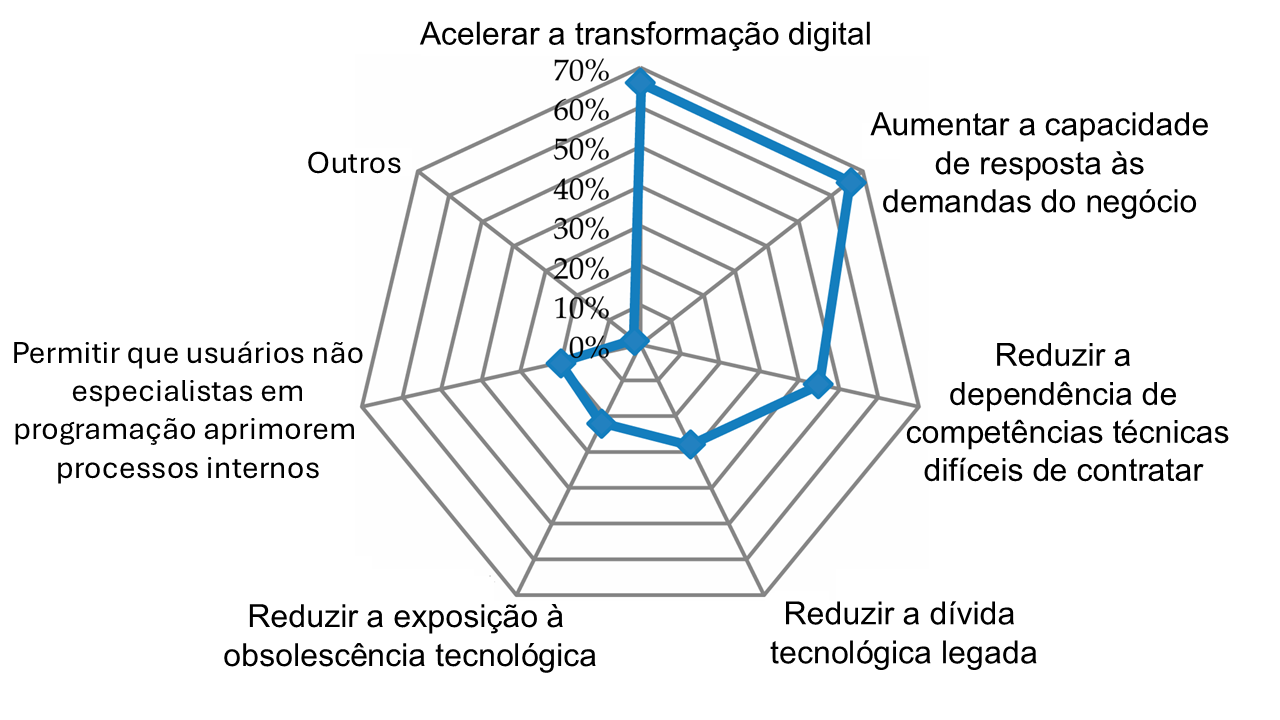
\includegraphics[width=0.78\textwidth]{Figuras/figura_motivos_low_code_pt.png}
\legend{Fonte: Adaptado de \citeonline[p.~3]{sanchis2020}.}
\end{figure}


% \dangersign[3ex] {\color{red}
% Não se esqueça de modificar o número de páginas antes da introdução (sem contar a capa)!
% No arquivo Monografia.tex altere a seguinte linha (no lugar de 14 coloque o valor contado de páginas): 
% $\backslash setcounter\{page\}\{11\} $% Inserir aqui o número de páginas antes da introdução menos a capa
% }


\section{Justificativa}

A manufatura contemporânea está inserida em um cenário de forte competitividade, no qual a eficiência operacional, a qualidade e a rapidez no acesso às informações tornaram-se fatores importantes para a gestão dos processos produtivos. Nesse contexto, a transformação digital passa a ter papel relevante, pois envolve o uso de tecnologias digitais para modificar produtos, processos e aspectos organizacionais, contribuindo para a competitividade e a geração de valor \cite[p.~1]{terra2022}. No ambiente industrial, essas mudanças também se relacionam ao aumento da produtividade, ao aprimoramento do controle da qualidade e à ampliação da flexibilidade operacional \cite[p.~1]{ribeiro2026}.

A justificativa deste trabalho está relacionada à necessidade de compreender como o uso de soluções digitais pode apoiar a organização e o acompanhamento de informações em processos industriais. Em rotinas produtivas, registros manuais ou pouco integrados podem dificultar a padronização dos dados, o acesso às informações e a análise das atividades realizadas. Além disso, a transformação digital nas organizações envolve alterações em processos produtivos, estrutura organizacional, competências, cultura e formas de gestão, desde que esteja alinhada à estratégia corporativa \cite[p.~57]{murici2022}. Dessa forma, analisar um caso real de manufatura permite observar como a digitalização pode contribuir para tornar as informações operacionais mais acessíveis e úteis à gestão.

Nesse cenário, as ferramentas \textit{low code} mostram-se adequadas ao tema deste estudo por possibilitarem maior agilidade na criação de aplicações e menor dependência de programação manual tradicional. Segundo Sanchis et al. \cite[p.~2]{sanchis2020}, essas plataformas utilizam interfaces visuais e elementos pré-configurados, permitindo maior participação de usuários ligados ao negócio no desenvolvimento de soluções digitais. Assim, este trabalho se justifica por analisar a aplicação de uma ferramenta \textit{low code} na digitalização de processos industriais, contribuindo para a compreensão de alternativas mais ágeis e adaptáveis para apoiar a gestão das informações no ambiente produtivo.



\section{Objetivos}

\subsection{\textit{Objetivo geral}}

O presente trabalho apresenta como objetivo geral analisar a digitalização de dois processos industriais em uma empresa de manufatura por meio da aplicação de uma ferramenta \textit{\textit{low code}}.

\subsection{\textit{Objetivos específicos}}

\begin{itemize}
\item Caracterizar os processos industriais analisados, considerando suas formas de registro, acompanhamento e organização das informações antes da digitalização.

\item Descrever a aplicação da ferramenta \textit{low code} nos processos estudados, observando sua utilização no contexto da empresa de manufatura.

\item Analisar as mudanças percebidas nos processos após a digitalização, considerando a acessibilidade, a padronização e a organização das informações.

\item Avaliar, a partir do estudo de caso, as contribuições da ferramenta \textit{low code} para o acompanhamento das rotinas operacionais e para a gestão das informações no ambiente produtivo.

\end{itemize}

\section{Organização do Texto}

No Capítulo 2 deste trabalho é apresentada a fundamentação teórica, abordando os principais conceitos relacionados à transformação digital, digitalização de processos industriais, manufatura e ferramentas \textit{low code}. No Capítulo 3 são descritos os procedimentos metodológicos utilizados para a realização do estudo de caso, considerando a caracterização da pesquisa, o ambiente analisado e as etapas adotadas para a análise dos processos. No Capítulo 4 são apresentados e discutidos os resultados obtidos a partir da análise da digitalização dos processos industriais estudados. Por fim, no Capítulo 5, são apresentadas as considerações finais do trabalho, destacando os principais resultados, limitações e sugestões para trabalhos futuros.


%Sugestões para estrutura da monografia:

% \begin{enumerate}[label=(\alph*)]
%   \item Introdução
%   \item Referencial Teórico (ou Revisão Bibliográfica)
%   \item Materiais e Métodos (ou Metodologia)
%   \item Resultados e Discussões
%   \item Conclusão (ou Considerações Finais)
%   \item Referências
% \end{enumerate}










\chapter{Fundamentação Teórica} \label{cap:FundamentacaoTeorica}


\section{Digitalização industrial e transformação digital}

A digitalização industrial pode ser compreendida como a conversão de atividades, registros e fluxos de informação, antes realizados de forma manual ou analógica, para meios digitais. No contexto da manufatura, essa mudança favorece a rastreabilidade, reduz limitações associadas ao preenchimento manual e facilita o acompanhamento das operações produtivas \cite{leite2024}.

A Transformação Digital (TD) possui um escopo mais amplo, pois envolve alterações nos processos, na estrutura organizacional e nas formas de gestão a partir do uso de tecnologias digitais \cite{murici2022}. Nesse sentido, a digitalização de processos industriais pode ser entendida como uma aplicação prática da TD no chão de fábrica, sobretudo quando orientada à melhoria da eficiência operacional, da qualidade e da tomada de decisão \cite{sanchis2020,ribeiro2026}.

\section{Indústria 4.0 e dados no ambiente de manufatura}

A Indústria 4.0 caracteriza-se pela integração de tecnologias digitais aos processos produtivos, possibilitando maior conexão entre máquinas, sistemas, pessoas e dispositivos. Nesse cenário, os dados assumem papel estratégico, pois apoiam o acompanhamento das operações, a análise de desempenho e a tomada de decisão, contribuindo para maior controle dos processos industriais \cite{sanchis2020,ribeiro2026}.

No contexto fabril, esses dados podem surgir de registros de produção, apontamentos operacionais, inspeções de qualidade, tempos de execução, ocorrências de falhas e informações coletadas por equipamentos conectados. Como observa \citeonline{rogers2016}, os dados podem ser gerados nas atividades internas da organização, como manufatura e operações, e utilizados em avaliações, previsões e decisões. Além disso, \citeonline{sanchis2020} associam o ambiente manufatureiro conectado à comunicação entre pessoas, aplicações e dispositivos de Internet das Coisas, o que amplia a disponibilidade e o uso dessas informações no processo produtivo.

A Transformação Digital 4.0, portanto, não depende apenas da adoção de ferramentas tecnológicas, mas também de condições organizacionais que sustentem o uso dos dados. \citeonline{leite2024} destacam dimensões como cultura digital, gestão da informação, infraestrutura tecnológica, operações estruturadas e desenvolvimento de competências digitais. Conforme a Figura~\ref{fig:dimensoes-td40}, esses elementos ajudam a visualizar como a digitalização industrial articula tecnologia, capacidade organizacional e uso das informações geradas no chão de fábrica.

\begin{figure}[htb]
    \centering
    \caption{Dimensões base para a Transformação Digital 4.0}
    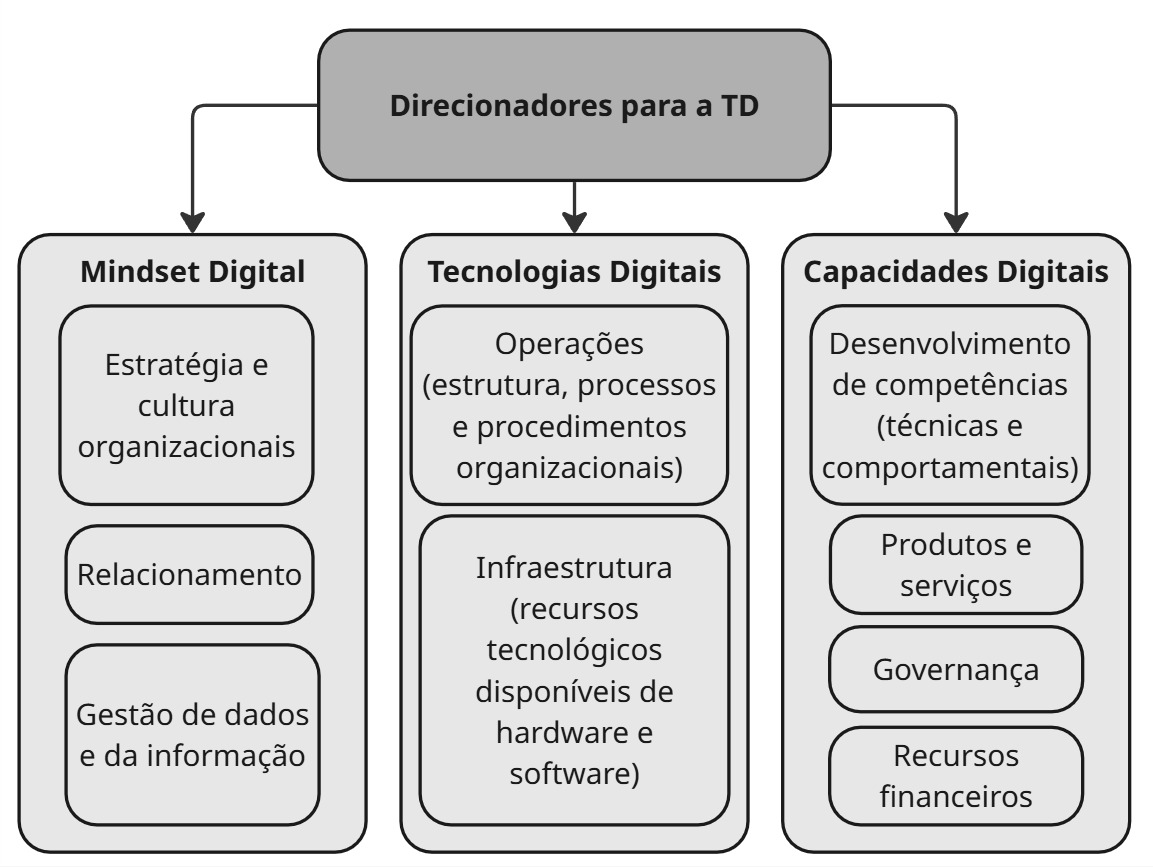
\includegraphics[width=0.85\textwidth]{Figuras/direcionadores_td.jpg}
    \label{fig:dimensoes-td40}
    
    \vspace{0.2cm}
    \begin{flushleft}
    \footnotesize Fonte: Elaborada pelo autor, com base em \citeonline{leite2024}.
    \end{flushleft}
\end{figure}

\section{Ferramentas low-code aplicadas à indústria}

As ferramentas \textit{low-code} podem ser compreendidas como plataformas de desenvolvimento que permitem a criação de aplicações digitais com menor dependência de codificação manual. Segundo \citeonline{sanchis2020}, essas plataformas utilizam interfaces visuais e componentes previamente estruturados, favorecendo o desenvolvimento rápido de aplicações. De forma complementar, \citeonline{alves2022} destacam que essa abordagem se apoia em abstrações de alto nível, diagramas visuais e linguagens declarativas, possibilitando menores tempos e custos quando comparada aos modelos tradicionais de desenvolvimento.

Na indústria, essa abordagem torna-se relevante por permitir que soluções digitais sejam desenvolvidas de forma mais flexível e próxima das demandas operacionais. Aplicações como formulários digitais, fluxos de aprovação, painéis de acompanhamento e integrações entre etapas produtivas podem ser construídas com maior agilidade. Com isso, o \textit{low-code} contribui para adaptar as soluções às rotinas do chão de fábrica e aos requisitos dos usuários envolvidos na operação \cite{sanchis2020,alves2022}.

Outro aspecto importante é a aproximação entre as áreas de negócio, processos e Tecnologia da Informação (TI). \citeonline{alves2022} apontam que o \textit{low-code} favorece a participação de profissionais que conhecem diretamente os procedimentos, desde a concepção até a validação das aplicações. Essa participação tende a gerar soluções mais aderentes à rotina operacional, especialmente em ambientes industriais nos quais o conhecimento prático do processo é essencial para definir fluxos, requisitos e informações necessárias.

Ao analisar plataformas \textit{low-code} de destaque, \citeonline{alves2022} comparam seus principais pontos fortes e limitações. Essa análise é relevante para este trabalho porque mostra que a escolha de uma plataforma não deve considerar apenas a rapidez de desenvolvimento, mas também aspectos como integração com sistemas existentes, colaboração entre usuários, gestão de fluxos, escalabilidade, manutenção e suporte a testes. O Quadro~\ref{quad:comparacao-lowcode} apresenta uma adaptação dessa comparação, relacionando características importantes para aplicações industriais.

\begin{quadro}[htb]
\centering
\caption{Comparação entre plataformas \textit{low-code}}
\label{quad:comparacao-lowcode}
\footnotesize
\begin{tabularx}{\textwidth}{>{\raggedright\arraybackslash}p{2.8cm}
                                >{\raggedright\arraybackslash}X
                                >{\raggedright\arraybackslash}X}
\hline
\textbf{Plataforma} & \textbf{Pontos fortes} & \textbf{Pontos de atenção} \\
\hline

Power Apps &
Integração com serviços em nuvem, uso de APIs personalizadas, suporte à política de dados, colaboração entre usuários e automação de fluxos de trabalho. &
Licenciamento complexo, menor suporte para desenvolvedores profissionais e restrições para compartilhamento externo. \\

\hline

OutSystems &
Boa experiência de usuário, escalabilidade, análise de desempenho e interoperabilidade. &
Poucos conectores externos, baixo suporte a estruturas de testes e ausência de desenvolvimento \textit{off-line}. \\

\hline

Mendix &
Suporte móvel \textit{off-line}, gerenciamento ágil de projetos, colaboração entre usuários e variedade de opções de implantação. &
Baixa integração com sistemas ERP, possíveis inconsistências em novas versões e custo elevado. \\

\hline

Salesforce Lightning &
Escalabilidade, recursos de teste, ferramentas associadas à inteligência artificial, gerenciamento amigável e serviço robusto. &
Possíveis instabilidades em integrações, maior necessidade de treinamento e menor nível de automação. \\

\hline

Appian &
Histórico agregado de processos, processamento de eventos complexos, colaboração simultânea, interfaces intuitivas e implantação rápida. &
Personalização limitada, depuração mais demorada e baixo suporte para testes. \\

\hline
\end{tabularx}

\vspace{0.2cm}
\begin{flushleft}
\footnotesize Fonte: Adaptado de \citeonline[p.~7--8]{alves2022}.
\end{flushleft}
\end{quadro}

O quadro reforça que as plataformas \textit{low-code} possuem características favoráveis à digitalização de processos industriais, principalmente quando o objetivo é transformar fluxos operacionais em aplicações digitais de uso prático. Para este estudo, destacam-se os recursos de integração, colaboração, automação de fluxos e disponibilização rápida das aplicações. Ao mesmo tempo, \citeonline{sanchis2020} chama atenção para desafios como escalabilidade, fragmentação entre plataformas e adequação a aplicações mais complexas. Assim, a adoção do \textit{low-code} deve ser acompanhada por análise do processo, validação com os usuários, acompanhamento das soluções implementadas e definição de critérios de governança \cite{sanchis2020,alves2022}.



\section{Aplicação digitalizada no estudo de caso}

\subsection{\textit{Resposta rápida para o controle da qualidade: 
conceito, funcionamento e aplicação}}

A Resposta Rápida para o Controle da Qualidade, conhecida pela sigla QRQC, do inglês \textit{Quick Response to Quality Control}, é utilizada para tratar problemas de qualidade de forma estruturada, com foco na reação rápida, na contenção do desvio, na análise da causa e na definição de ações corretivas capazes de evitar a reincidência da falha. Segundo \citeonline{rocha2012}, o QRQC é uma metodologia de gerenciamento à vista que reúne ferramentas da qualidade para apoiar a análise e a identificação de problemas no processo produtivo.

A aplicação do QRQC está associada à necessidade de resolver problemas diretamente na fonte, com base em fatos, evidências e participação dos envolvidos no processo. Para \citeonline{rocha2012}, a metodologia utiliza ferramentas como 5W2H, Diagrama de Ishikawa, 5 Porquês e Diagrama de Pareto, aplicadas de forma sequencial para auxiliar na contenção do problema e na investigação das causas. Dessa forma, o QRQC contribui para organizar a tratativa das não conformidades e tornar mais clara a relação entre o problema identificado, suas causas e as ações necessárias.

O funcionamento da metodologia pode ser compreendido como um fluxo de resposta rápida que começa pela identificação do problema e pela adoção de ações imediatas de contenção. Em seguida, são analisados os riscos de ocorrência em outros produtos ou processos, investigadas as causas da falha e da não detecção, definidas ações corretivas e verificada a efetividade das soluções adotadas. \citeonline{moreira2023} relaciona essa lógica às etapas da metodologia 8D, envolvendo definição do problema, análise de risco, contenção, identificação das causas, ações corretivas, verificação e registro das lições aprendidas.

No ambiente industrial, a aplicação do QRQC depende da integração entre pessoas, registros e informações do processo. A participação dos colaboradores que atuam diretamente na operação é importante porque permite que a análise considere o local real da ocorrência, as condições do processo e as evidências disponíveis. Nesse sentido, \citeonline{moreira2023} destaca que o comprometimento dos envolvidos e da gestão é essencial para que a metodologia contribua para a melhoria contínua e para o tratamento adequado dos problemas de qualidade.

No contexto deste estudo, o QRQC é as aplicação digitalizada porque envolve informações que precisam ser registradas, acompanhadas e atualizadas ao longo da tratativa da não conformidade. Entre essas informações, podem estar a descrição do problema, a área responsável, as ações de contenção, os prazos, os responsáveis, as evidências, as causas identificadas e a verificação da eficácia das ações. Assim, a digitalização desse processo pode apoiar a rastreabilidade das ocorrências, a padronização dos registros e o acompanhamento das ações em andamento, aproximando a metodologia de resposta rápida das práticas de gestão da informação no ambiente de manufatura.


\section{Barreiras e cuidados na digitalização de processos industriais}

A digitalização de processos industriais pode contribuir para a organização das informações, o acompanhamento das atividades e a tomada de decisão. No entanto, sua implantação exige cuidados que vão além da escolha da ferramenta tecnológica. \citeonline{murici2022} destaca que a Transformação Digital envolve mudanças em processos, estrutura, cultura, competências e formas de gestão, o que evidencia a necessidade de considerar também os fatores humanos e organizacionais.

Entre as principais barreiras, estão a resistência à mudança, a carência de pessoal qualificado, o despreparo dos usuários e a dificuldade de adaptação a novos fluxos de trabalho \cite{murici2022}. No ambiente de manufatura, esses fatores podem interferir diretamente no uso das aplicações digitais, especialmente quando há substituição de registros manuais por formulários eletrônicos, necessidade de padronização dos dados e acompanhamento das informações em tempo real.

Também devem ser considerados aspectos técnicos e de governança. Embora as plataformas \textit{low-code} favoreçam o desenvolvimento rápido de aplicações, \citeonline{sanchis2020} apontam desafios relacionados à escalabilidade, fragmentação entre plataformas e adequação a aplicações mais complexas. Dessa forma, a digitalização de processos industriais deve ser acompanhada por análise do processo, validação com os usuários, definição de responsabilidades, controle dos dados e manutenção das soluções implementadas \cite{alves2022}.






% \section{Acrescentando um arquivo tex na estrutura}

Como acrescentar uma nova subseção, utilizando um arquivo externo:

\begin{enumerate}
    \item crie um arquivo .tex (ex.: meuarquivo.tex)
    \item Se for um arquivo de capítulo:
        \subitem No arquivo Monografia.text acrescente a seguinte linha na ordem que deseja aparecer no texto: $\backslash include\{Capitulos/meuarquivo\}$
    \item Se for parte do texto:
        \subitem Inserir no arquivo onde se deseja continuar o seguinte comando:
            \subsubitem $\backslash input\{Capitulos/meuarquivo\}$
    
    
\end{enumerate}


{\color{blue}

Obs.: Este texto foi escrito no arquivo exemplo subsecao2.tex. 
Note que o arquivo é inserido em continuidade na página!

}
 % a ordem é a que aparece no texto






\chapter{Metodologia}
\label{cap:metodologia}

\section{Caracterização da pesquisa}
\label{sec:caracterizacao}

Quanto à natureza, a pesquisa é aplicada, pois trata de um problema concreto: a organização do registro e do acompanhamento das informações do QRQC em uma rotina industrial. Quanto aos objetivos, é descritiva, uma vez que busca registrar como a aplicação estrutura esse processo e como os dados por ela gerados são apresentados, sem estabelecer relações de causa e efeito \cite{prodanov2013}.

Quanto à abordagem, a pesquisa combina elementos qualitativos e quantitativos. A parte qualitativa consiste no exame das páginas, do modelo de dados e das regras da aplicação, interpretados à luz das etapas do QRQC descritas na literatura. A parte quantitativa consiste na descrição dos indicadores do QRQC apresentados em uma ferramenta de \textit{Business Intelligence} (BI), alimentada pelos registros da própria aplicação \cite{prodanov2013}.

Quanto aos procedimentos, adota-se o estudo de caso único, adequado quando se pretende examinar um fenômeno contemporâneo em seu contexto real, com o apoio de múltiplas fontes de evidência \cite{yin2018}. O caso é o QRQC digitalizado por meio de uma aplicação desenvolvida em Mendix. A unidade de análise é essa aplicação, examinada em sua totalidade quanto ao suporte que oferece às etapas do QRQC; funcionalidades de apoio, como cadastros de usuários e de tipos de defeito, são consideradas na medida em que sustentam o registro e o acompanhamento das ocorrências.

O estudo não compara o processo antes e depois da implantação da aplicação, pois não há registros suficientes sobre a rotina anterior. Assim, os indicadores obtidos no BI descrevem o funcionamento do processo no período analisado, mas não permitem afirmar que a digitalização tenha provocado melhorias de desempenho. A organização é identificada por nome fictício, e os dados apresentados são anonimizados.

\chapter{Resultados e discussão}
\label{cap:resultados}

\chapter{Considerações finais}
\label{cap:conclusao}




% ----------------------------------------------------------
% -- Elementos Pós-Textuais: -------------------------------
\postextual  
\citeoption{abnt-opcoes}
\bibliographystyle{packages/abntex2-alf}
\bibliography{bibliografia} % Referências bibliográficas
% Habilitar apenas apêndices e anexos efetivamente utilizados.
% Apêndice A - Fluxogramas baseados nos microflows da aplicação
% Requer \usepackage{pdflscape} e \usetikzlibrary{shapes.geometric,calc,fit} no preâmbulo.

\begin{apendicesenv}
\chapter{Lógica de salvamento de uma ocorrência}
\label{ap:salvar}

Este apêndice apresenta a lógica executada quando o usuário salva a descrição do problema de uma nova ocorrência, modelada no Mendix em \textit{microflows} (Seção~\ref{sec:mendix}). Em vez de capturas de tela, optou-se por fluxogramas elaborados pelo autor, por dois motivos: os originais trazem nomes em inglês e detalhes de implementação que dificultariam a leitura, e seus nomes de módulos e entidades permitiriam identificar a organização. Os fluxogramas mantêm a sequência de atividades e decisões, com nomes traduzidos e generalizados.

Antes de gravar o registro, a aplicação valida os campos obrigatórios da descrição do problema, em cinco grupos de verificação, como mostra a Figura~\ref{fig:mf-validar}. Basta um campo pendente para que a ocorrência não seja salva, e a mensagem aparece junto ao campo correspondente.

Concluída a validação, o fluxo principal (Figura~\ref{fig:mf-salvar}) gera o identificador da ocorrência ou, se ela era um rascunho, muda sua situação para aberta. Em seguida, envia o registro ao sistema de controle de \textit{tickets}, que devolve o número do chamado, avança a ocorrência para a ação de contenção, carrega a configuração de verificação da unidade, registra o histórico, vincula os anexos e salva a ocorrência. Por fim, aciona a sirene e dispara as notificações. Se a validação ou a integração falharem, nada é salvo, e por isso não existe ocorrência sem um chamado vinculado.

\begin{figure}[htbp]
    \centering
    \caption{Fluxograma baseado no \textit{microflow} de validação da descrição do problema}
    \label{fig:mf-validar}
    \resizebox{\textwidth}{!}{%
    \begin{tikzpicture}[fx, fxproc/.append style={text width=3.0cm, minimum width=3.3cm}]
    \simbolosFX{-4.4,0.4}{fxtermleg/Terminal, fxdecleg/Decisão, fxprocleg/Processamento, fxconleg/Conector}{4}
    % ---------- coluna 1
    \node[fxterm] (ini) at (0,0) {Início};
    \node[fxproc, below=of ini] (v1) {Verificar tipo e descrição: tipo preenchido e descrição do problema preenchida};
    \node[fxdec, below=of v1] (d1) {Tipo e descrição OK?};
    \node[fxproc, below=of d1] (v2) {Verificar local e responsável pela detecção: no tipo segurança, formulário de segurança; nos demais, detectado por, turno, cliente, linha, produto e revisão e sintoma};
    \node[fxdec, below=of v2] (d2) {Detecção OK?};
    \node[fxcon, below=of d2] (c1) {1};
    \node[fxcon] (e1) at ($(d1)+(2.5,0)$) {2};
    \node[fxcon] (e2) at ($(d2)+(2.5,0)$) {2};
    % ---------- coluna 2
    \node[fxcon] (c1b) at (5.4,0) {1};
    \node[fxproc, below=of c1b] (v3) {Verificar a dimensão do problema: frequência e quantidade preenchidas};
    \node[fxdec, below=of v3] (d3) {Dimensão OK?};
    \node[fxproc, below=of d3] (v4) {Verificar a categoria: ao menos uma assinalada; se ``outros'', descrição obrigatória};
    \node[fxdec, below=of v4] (d4) {Categoria OK?};
    \node[fxcon, below=of d4] (c2) {3};
    \node[fxcon] (e3) at ($(d3)+(2.5,0)$) {2};
    \node[fxcon] (e4) at ($(d4)+(2.5,0)$) {2};
    % ---------- coluna 3
    \node[fxcon] (c2b) at (10.8,0) {3};
    \node[fxproc, below=of c2b] (v5) {Verificar os cadastros: cliente e unidade existentes};
    \node[fxdec, below=of v5] (d5) {Cadastros OK?};
    \node[fxterm, below=of d5] (ok) {Fim: descrição válida};
    \node[fxcon] (e5) at ($(d5)+(2.5,0)$) {2};
    \node[fxcon, below=of ok] (eb) {2};
    \node[fxterm, below=of eb] (erro) {Fim: mensagem junto ao campo pendente; nada é salvo};
    \foreach \a/\b in {ini/v1, v1/d1, v2/d2, c1b/v3, v3/d3, v4/d4, c2b/v5, v5/d5, eb/erro} { \draw[fxseta] (\a) -- (\b); }
    \foreach \a/\b in {d1/v2, d2/c1, d3/v4, d4/c2, d5/ok} { \draw[fxseta] (\a) -- node[fxrot, left, pos=0.4]{Sim} (\b); }
    \foreach \a/\b in {d1/e1, d2/e2, d3/e3, d4/e4, d5/e5} { \draw[fxseta] (\a) -- node[fxrot, above, pos=0.4]{Não} (\b); }
    \node[fxquadro, fit=(current bounding box)] {};
    \end{tikzpicture}}
    \legend{Fonte: elaborado pelo autor (2026), com base no \textit{microflow} de validação da aplicação, no Mendix Studio Pro.}
\end{figure}

\begin{landscape}
\begin{figure}[p]
    \centering
    \caption{Fluxograma baseado no \textit{microflow} de salvamento de uma ocorrência}
    \label{fig:mf-salvar}
    \resizebox{\linewidth}{!}{%
    \begin{tikzpicture}[fx]
    \simbolosFX{-4.3,0.4}{fxtermleg/Terminal, fxdecleg/Decisão, fxprocleg/Processamento, fxsubleg/Subprocesso, fxconleg/Conector}{5}
    % ---------- coluna 1
    \node[fxterm] (ini) at (0,0) {Início};
    \node[fxsub, below=of ini] (val) {Validar a descrição do problema (Figura~\ref{fig:mf-validar})};
    \node[fxdec, below=of val] (ok) {Campos válidos?};
    \node[fxfim, text width=1.6cm, minimum width=1.8cm] (f1) at ($(ok)+(3.1,0)$) {Fim: nada é salvo};
    \node[fxdec, below=of ok] (rasc) {Era um rascunho?};
    \node[fxproc, below=of rasc] (id) {Gerar o identificador da ocorrência};
    \node[fxproc] (aberta) at ($(id)+(3.4,0)$) {Mudar a situação para aberta};
    \node[fxcon, below=0.9cm of id] (c1) {1};
    \coordinate[below=0.4cm of id] (m1);
    \draw[fxseta] (ini) -- (val);
    \draw[fxseta] (val) -- (ok);
    \draw[fxseta] (ok) -- node[fxrot, above, pos=0.4]{Não} (f1);
    \draw[fxseta] (ok) -- node[fxrot, left, pos=0.4]{Sim} (rasc);
    \draw[fxseta] (rasc) -- node[fxrot, left, pos=0.4]{Não} (id);
    \draw[fxseta] (rasc.east) -- node[fxrot, above, pos=0.3]{Sim} (rasc.east -| aberta) -- (aberta);
    \draw (id) -- (m1);
    \draw (aberta.south) |- (m1);
    \draw[fxseta] (m1) -- (c1);
    % ---------- coluna 2
    \node[fxcon] (c1b) at (7.3,0) {1};
    \node[fxproc, below=of c1b] (desc) {Gerar a descrição resumida};
    \node[fxsub, below=of desc] (post) {Enviar ao sistema de \textit{tickets} e receber o número do chamado};
    \node[fxdec, below=of post] (suc) {Chamado criado?};
    \node[fxcon] (c2) at ($(suc)+(2.4,0)$) {2};
    \node[fxproc, below=of suc] (log) {Registrar o erro};
    \node[fxfim, below=of log] (f2) {Fim};
    \foreach \a/\b in {c1b/desc, desc/post, post/suc, log/f2} { \draw[fxseta] (\a) -- (\b); }
    \draw[fxseta] (suc) -- node[fxrot, above, pos=0.4]{Sim} (c2);
    \draw[fxseta] (suc) -- node[fxrot, left, pos=0.4]{Não} (log);
    % ---------- coluna 3
    \node[fxcon] (c2b) at (11.9,0) {2};
    \node[fxproc, below=of c2b] (cont) {Avançar para a ação de contenção};
    \node[fxproc, below=of cont] (conf) {Carregar a configuração de verificação da unidade};
    \node[fxproc, below=of conf] (hist) {Registrar o histórico e a configuração da ocorrência};
    \node[fxproc, below=of hist] (anexo) {Vincular os anexos à ocorrência};
    \node[fxcon, below=of anexo] (c3) {3};
    \foreach \a/\b in {c2b/cont, cont/conf, conf/hist, hist/anexo, anexo/c3} { \draw[fxseta] (\a) -- (\b); }
    % ---------- coluna 4
    \node[fxcon] (c3b) at (15.6,0) {3};
    \node[fxdec, below=of c3b] (temid) {Identificador gerado?};
    \node[fxfim] (f3) at ($(temid)+(2.5,0)$) {Fim};
    \node[fxproc, below=of temid] (salva) {Salvar a ocorrência};
    \node[fxproc, below=of salva] (msg) {Exibir a confirmação ao usuário};
    \node[fxcon, below=of msg] (c4) {4};
    \draw[fxseta] (c3b) -- (temid);
    \draw[fxseta] (temid) -- node[fxrot, above, pos=0.4]{Não} (f3);
    \draw[fxseta] (temid) -- node[fxrot, left, pos=0.4]{Sim} (salva);
    \foreach \a/\b in {salva/msg, msg/c4} { \draw[fxseta] (\a) -- (\b); }
    % ---------- coluna 5
    \node[fxcon] (c4b) at (21.2,0) {4};
    \node[fxproc, below=of c4b] (sir) {Acionar a sirene};
    \node[fxsub, below=of sir] (not) {Enviar notificações: e-mail aos envolvidos e alerta aos painéis};
    \node[fxterm, below=of not] (fim) {Fim};
    \foreach \a/\b in {c4b/sir, sir/not, not/fim} { \draw[fxseta] (\a) -- (\b); }
    \node[fxquadro, fit=(current bounding box)] {};
    \end{tikzpicture}}
    \legend{Fonte: elaborado pelo autor (2026), com base no \textit{microflow} de salvamento da aplicação, no Mendix Studio Pro.}
\end{figure}
\end{landscape}

\chapter{Esquema elétrico de acionamento da sirene}\label{ap:sirene}

A Figura~\ref{fig:esquema-sirene} apresenta o esquema elétrico usado para acionar a sirene a partir da aplicação, integração descrita na Seção~\ref{subsec:integracoes}. A parte superior da figura mostra a pinagem do Raspberry Pi, com o GPIO22 destacado em verde, e a parte inferior mostra a ligação entre os componentes. Quando uma ocorrência é criada, ou quando o botão de sirene do painel é acionado, a aplicação envia um comando por API REST ao Raspberry Pi instalado na área produtiva. O Raspberry Pi coloca em nível alto a saída GPIO22 (pino físico 15), que é o pino padrão do acionamento e não pode ser alterado. Essa saída comanda a entrada do módulo de relé, alimentado pelos pinos de alimentação (VCC) e terra (GND) do próprio Raspberry Pi.

Com o relé energizado, o contato comum (C) fecha com o contato normalmente aberto (NA) e a fonte de alimentação passa a alimentar a sirene; quando a saída volta a nível baixo, o contato abre e a sirene desliga. O relé separa o circuito lógico do Raspberry Pi, de baixa corrente, do circuito de potência da sirene, que tem alimentação própria. Assim, a corrente da sirene não circula pela saída do Raspberry Pi, que apenas comanda o relé. O esquema apresenta apenas a lógica de ligação, para delimitar o escopo da solução: as tensões, as correntes e os modelos dos componentes foram omitidos propositalmente, pois dependem da sirene e da fonte adotadas em cada instalação. Para a implementação, devem ser consultados os manuais dos componentes escolhidos e verificada a compatibilidade entre eles. A sinaleira, também acionada a cada ocorrência criada (Seção~\ref{subsec:integracoes}), é ligada ao mesmo relé e, por isso, é acionada junto com a sirene; ela não foi representada separadamente no esquema.

\begin{figure}[htbp]
    \centering
    \caption{Esquema elétrico de acionamento da sirene}\label{fig:esquema-sirene}
    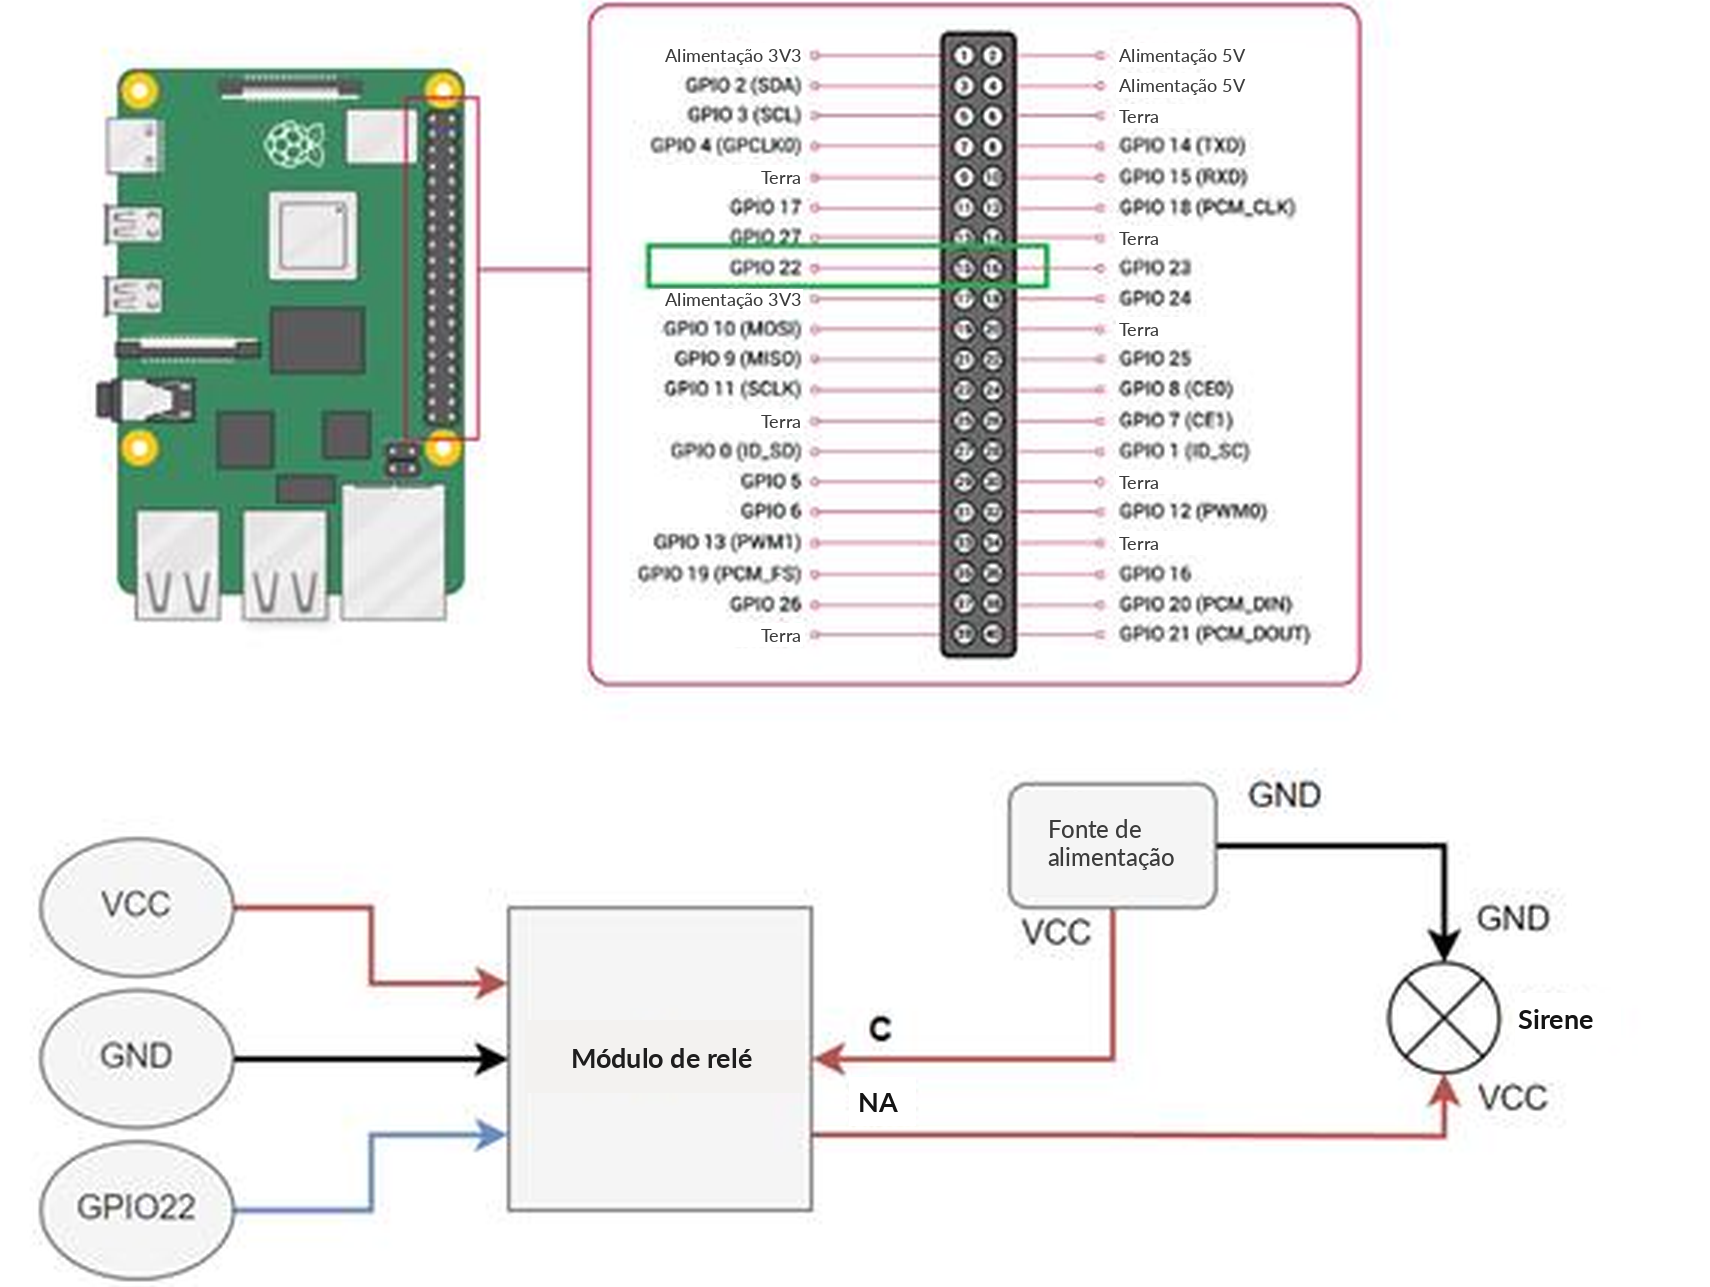
\includegraphics[width=0.95\textwidth]{Figuras/esquema-sirene.png}
    \legend{Fonte: documentação interna da aplicação, traduzido pelo autor (2026).}
\end{figure}
\end{apendicesenv}

% %----------------------------------------------------------------
%---------------------- Anexos ----------------------------------
%----------------------------------------------------------------

\begin{anexosenv}
%\partanexos   % indica o início dos anexos
\chapter{Mapa de unidades do IFMG.}
\label{anexoA}

Note que os  Anexos são  \textbf{documentos  que não foram  elaborados  pelo  autor},  que  servem  também  de  fundamentação, comprovação ou ilustração do trabalho, como leis, mapas, ilustrações etc .

\begin{figure}[H] % h! para here, b para bottom e t para top
   \begin{center}
    \caption{Mapa de unidades do IFMG.} %//não esqueça o ponto final
    \label{fig:mapas}
    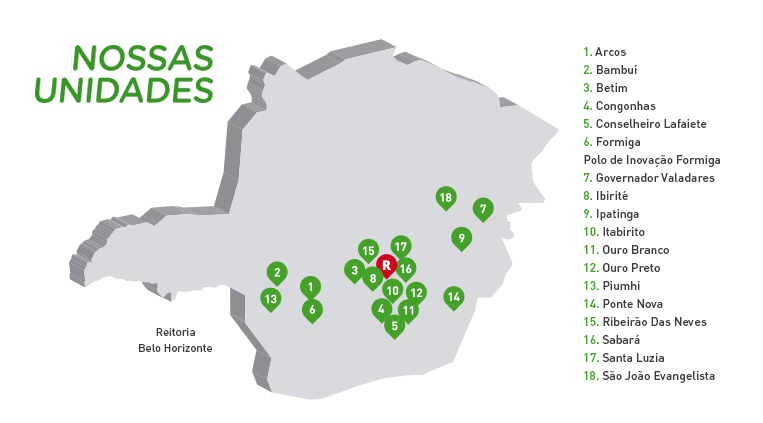
\includegraphics[width=1\linewidth]{Figuras/mapasitenovonov2018b.png} \\
    \end{center}
    \fontsize{10}{12}\selectfont{Fonte: \href{https://www.ifmg.edu.br/portal/sobre-o-ifmg/mapasitenovonov2018b.png}{https://www.ifmg.edu.br/portal/sobre-o-ifmg}. }
\end{figure}



\end{anexosenv}

%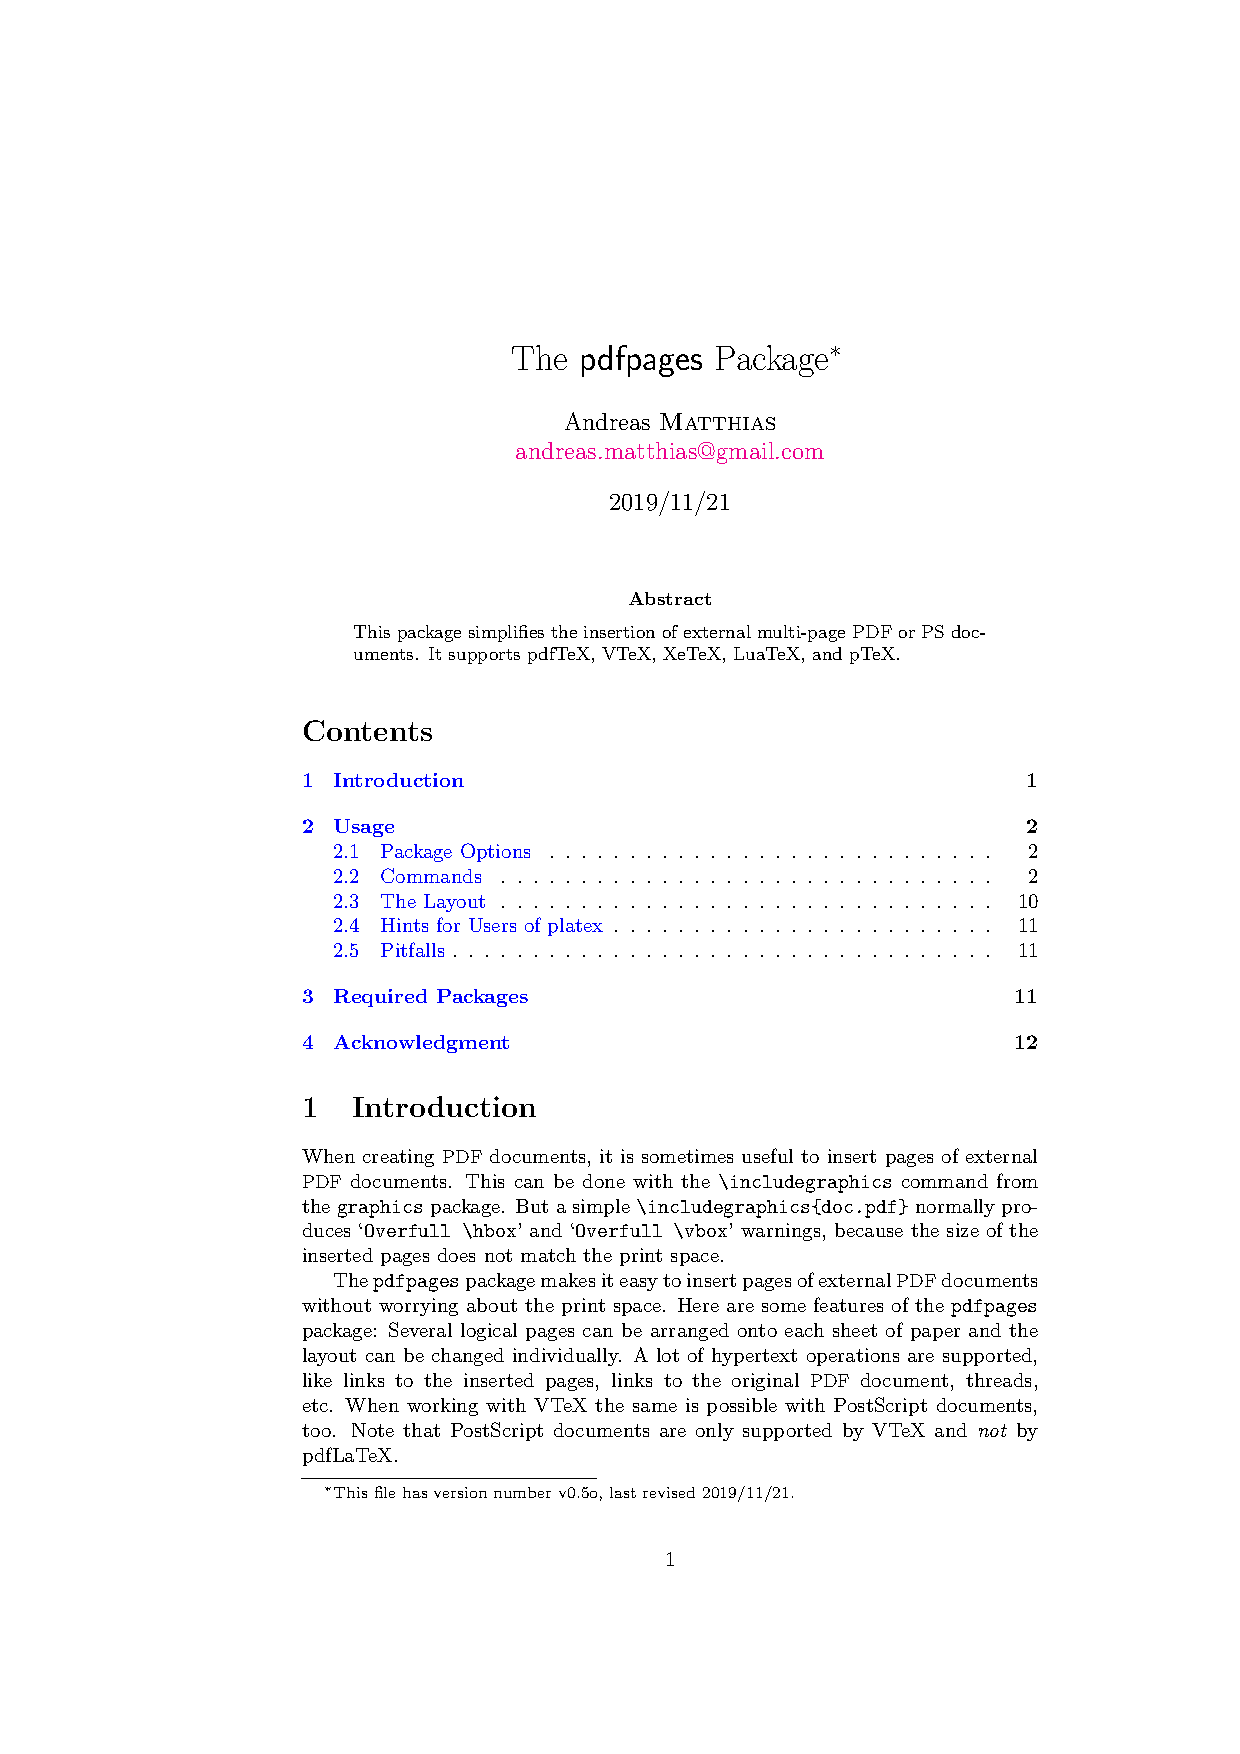
\includepdf[pages={1,3-5}]{PosTextuais/includepdfpages.pdf}
%\phantompart  \printindex  % Indice Remissivo
% ----------------------------------------------------------
\end{document}  % fim do documento
